\chapter{Results}
\section{Content Analysis Results}
From the retrospective reports we obtained several interesting results. We will go through each of them below starting with some key numbers and then move on to the results of the content analysis. Then we identify some trends observed while performing the content analysis. 

\subsection{Key Numbers}
In this section we will present some key numbers of the retrospective results and this numbers can also be seen in \autoref{table:key-numbers}.

\begin{table}[!h]
	\begin{center}
	\caption{Some key numbers from the retrospectives}
	\label{table:key-numbers}
	\makebox[\textwidth]{%
		\begin{tabular}{ l | p{0.5\textwidth}}
		\hline
		Key-value & Value  \\
		\hline
		Retrospective report period & 278 Weeks \\
		Number of total actions & 343 \\
		Number of unresolved actions & 65 \\
		Average actions per week & 1.23 \\
		Average unresolved action per week & 0.23 \\
		\hline
		\end{tabular}
	}
\end{center}
\end{table}

The retrospective reports spanned over a period of five years from August 2009 to November 2014. This is equal to 278 weeks and we are going to refer to week numbers from the first retrospective for the remainder of this report. 
During the 278 weeks 77 retrospectives were held and and within these 343 actions was created, where 65 of these actions were still unresolved. This yields an average of 4.45 actions per retrospective and 0.84 unresolved per retrospective. This is equal to 1.23 actions per week, where one have 0.23 unresolved actions per week. 

\begin{sidewaysfigure}[!h]
	\centering
	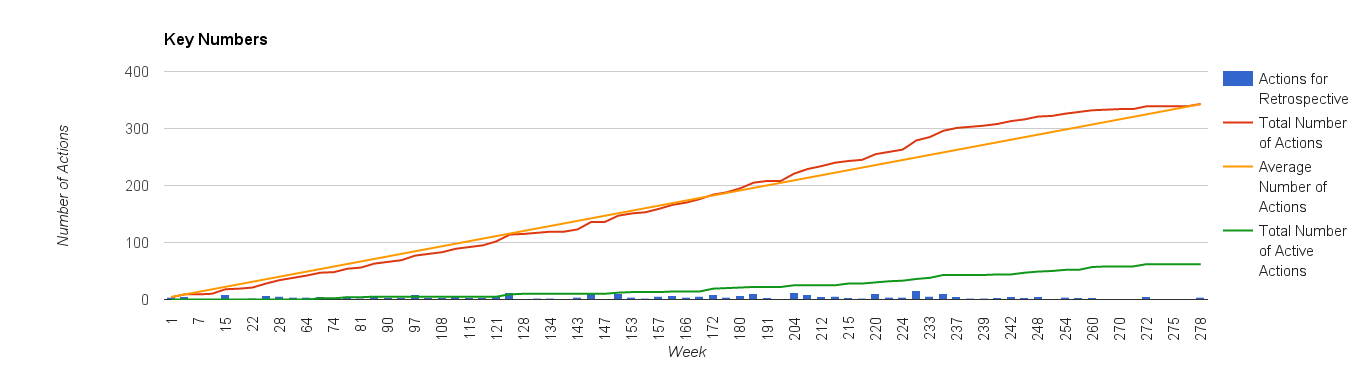
\includegraphics[width=\textwidth]{figures/key-numbers.png}
	\caption{A visual representation of some of the key numbers.}
	\label{figure:key-numbers}
\end{sidewaysfigure}
\afterpage{\clearpage}

In \autoref{figure:key-numbers} we can see the development of numbers of actions. We can see that the team has had a pretty steady amount of actions with no abnormal spikes or changes. The total amount of actions follows the average expected actions quite close and reveals the steady number of actions. The amount of active (or unresolved) actions also has a steady amount of total actions increasing at about the same rate as the total number of actions. 

\subsection{Analysis Results}
In this section we will present the results from our content analysis. We will present the results for each theme defined in \autoref{method:categories}. 

\subsubsection{Nature}
The content analysis revealed that most actions are created as a result of negative problems that has occurred during the development. 89.3\% of the actions were negative, while 5.5\% of the actions were positive and acknowledged good working practices that would be continued. 5.2\% of the actions we lacked the context to determine whether they were positive or negative. As for the distribution of the actions over each retrospective there was no abnormalities except week 97 where there was an unusual amount of positive actions. However while looking into this week we found nothing in particular that could be identified as cause for this spike. As can be seen in \autoref{figure:nature-pa} and \autoref{table:nature-results} the classification of the active actions pretty much mirrored the results from the total actions. 

\begin{table}[!h]
	\begin{center}
	\caption{Analysis results from the content analysis for the nature of the action.}
	\label{table:nature-results}
	\makebox[\textwidth]{%
		\begin{tabular}{| l | l | l | l | l |}
		\hline
		Category & \multicolumn{2}{|c|}{All Actions} & \multicolumn{2}{|c|}{Active Actions}  \\
		\cline{2-5}
		& Number & Percentage & Number & Percentage \\	
		\hline
		Positive & 19 & 5.5\% & 1 & 1.6\% \\
		Negative & 310 & 89.3\% & 57 & 90.5\% \\
		Undefined & 18 & 5.2\% & 5 & 7.9\% \\
		\hline
		\end{tabular}
	}
	\end{center}
\end{table}

\begin{figure}[!h]
	\centering
	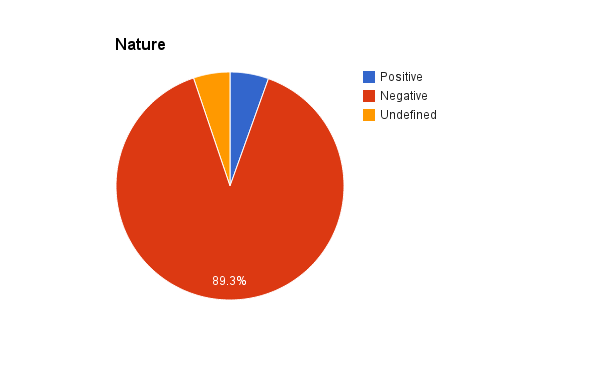
\includegraphics[width=\textwidth]{figures/nature-p.png}
	\caption{The negative, positive and undefined distribution of all the actions.}
	\label{figure:nature-p}
\end{figure}

\begin{figure}[!h]
	\centering
	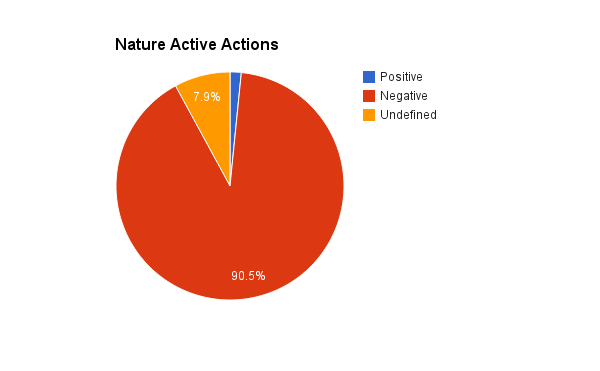
\includegraphics[width=\textwidth]{figures/nature-pa.png}
	\caption{The negative, positive and undefined distribution of the active actions.}
	\label{figure:nature-pa}
\end{figure}

\begin{sidewaysfigure}[!h]
	\centering
	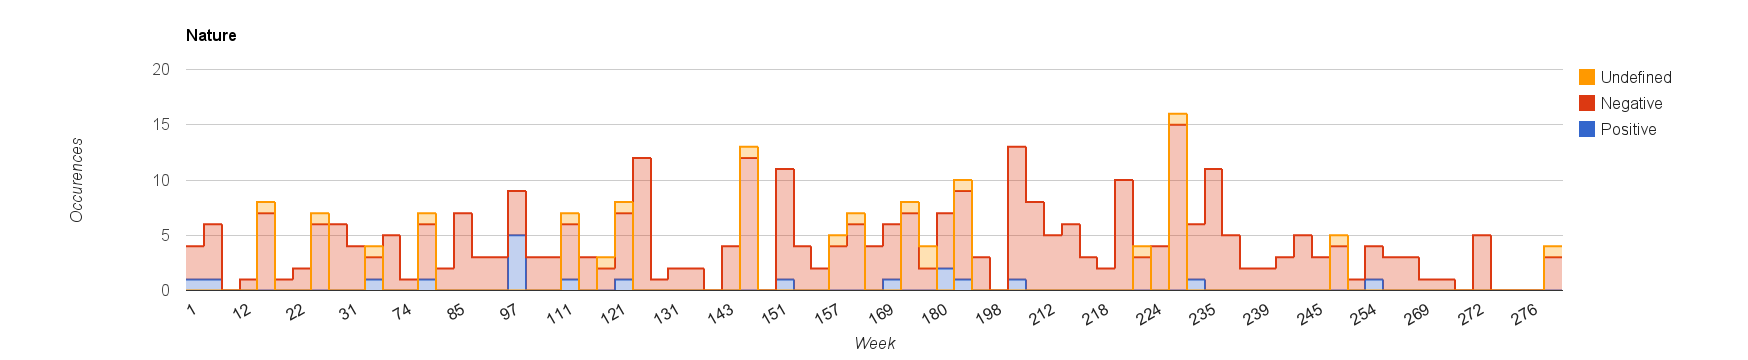
\includegraphics[width=\textwidth]{figures/nature-l.png}
	\caption{The distribution of negative, positive and undefined actions across the timespan}
	\label{figure:nature-l}
\end{sidewaysfigure}

\afterpage{\clearpage}

\subsubsection{Context}
For the context of the actions analyzed mostly where process related ones. The process actions numbered in 228, which is equal to 58.6\% of all the actions. The Technical ones numbered as 157 which is 40.4\%, while only 4 actions were undefined which results in 1\% of the total actions. As for the distribution over the timespand analyzed there where no abnormalities as can be seen in \autoref{figure:context-l}. For the active actions the results become more equal as seen in \autoref{figure:context-pa}. However it is worth mentioning that the active actions are a sub-group of the total and thus this result is probably a skewed grouping. 

\begin{table}[!h]
	\begin{center}
	\caption{Analysis results from the content analysis for the context of the action.}
	\label{table:context-results}
	\makebox[\textwidth]{%
		\begin{tabular}{| l | l | l | l | l |}
		\hline
		Category & \multicolumn{2}{|c|}{All Actions} & \multicolumn{2}{|c|}{Active Actions}  \\
		\cline{2-5}
		& Number & Percentage & Number & Percentage \\	
		\hline
		Technical & 157 & 40.4\% & 37 & 52.1\% \\
		Process & 228 & 58.6\% & 34 & 47.9\% \\
		Undefined & 4 & 1\% & 0 & 0\% \\
		\hline
		\end{tabular}
	}
	\end{center}
\end{table}

\begin{figure}[!h]
	\centering
	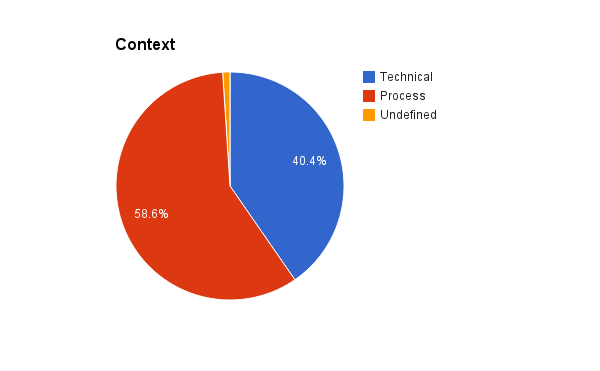
\includegraphics[width=\textwidth]{figures/context-p.png}
	\caption{The distribution of technical, process and undefined related actions.}
	\label{figure:context-p}
\end{figure}

\begin{figure}[!h]
	\centering
	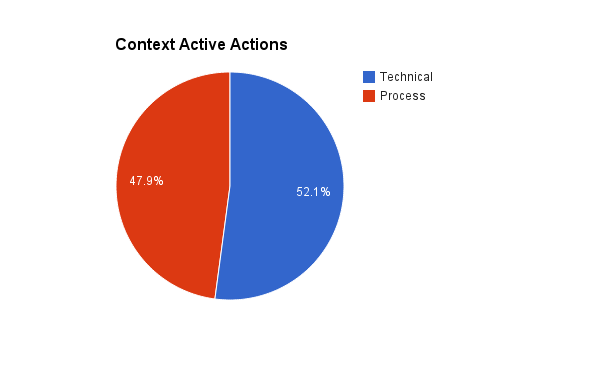
\includegraphics[width=\textwidth]{figures/context-pa.png}
	\caption{The distribution of technical, process and undefined related actions over.}
	\label{figure:context-pa}
\end{figure}

\begin{sidewaysfigure}[!h]
	\centering
	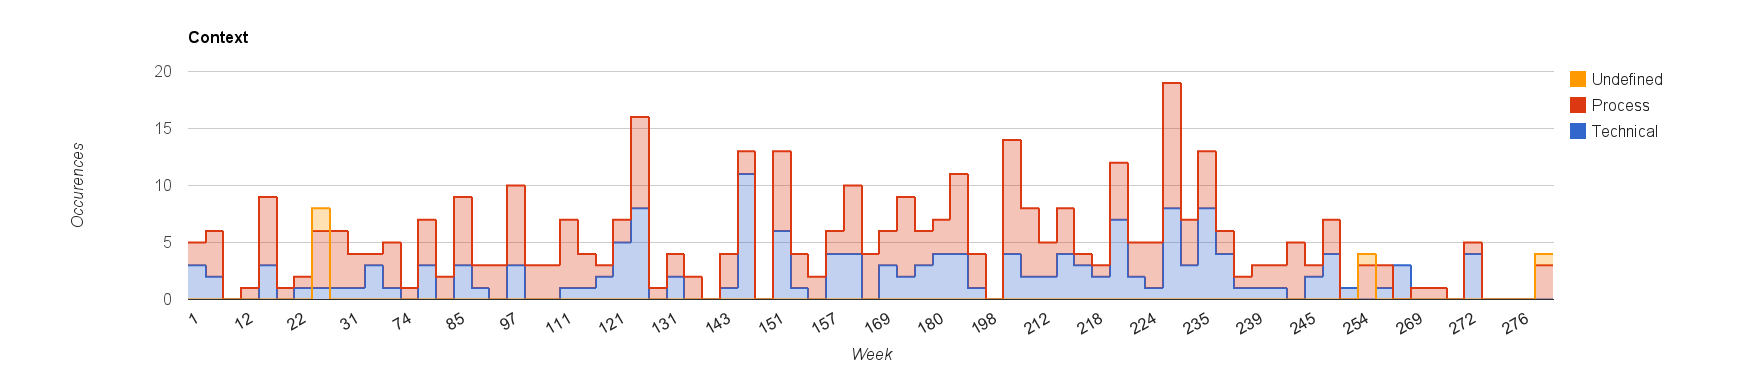
\includegraphics[width=\textwidth]{figures/context-l.png}
	\caption{The distribution of technical, process and undefined related actions across the timespan.}
	\label{figure:context-l}
\end{sidewaysfigure}

\afterpage{\clearpage}

\subsubsection{Decision Making}
The decision making results showed that the operational decision occurred most in the actions as can be seen in \autoref{table:decision-making-results} and \autoref{figure:decision-p}. Operational decisions occurred in 53.2\% of the actions, while tactical was at 25.9\% and strategic was at 16.1\% of the actions. There only was four cases where we were not able to determine which kinds of decision making type it was. For the distribution over time, as shown in \autoref{figure:decision-l}, there was no emerging patterns and all the decision making types was evenly distributed. The active actions mirrored the total actions almost equal as can be seen in \autoref{figure:decision-p} and \autoref{figure:decision-pa}.

\begin{table}[!h]
	\begin{center}
	\caption{Analysis results from the content analysis for the decision making perspective of the action.}
	\label{table:decision-making-results}
	\makebox[\textwidth]{%
		\begin{tabular}{| l | l | l | l | l |}
		\hline
		Category & \multicolumn{2}{|c|}{All Actions} & \multicolumn{2}{|c|}{Active Actions}  \\
		\cline{2-5}
		& Number & Percentage & Number & Percentage \\	
		\hline
		Strategic & 55 & 16\% & 10 & 16.1\% \\
		Tactical & 89 & 25.9\% & 18 & 29\% \\
		Operational & 195 & 56.9\% & 33 & 53.2\% \\
		Undefined & 4 & 1.2\% & 1 & 1.6\% \\
		\hline
		\end{tabular}
	}
	\end{center}
\end{table}

\begin{figure}[!h]
	\centering
	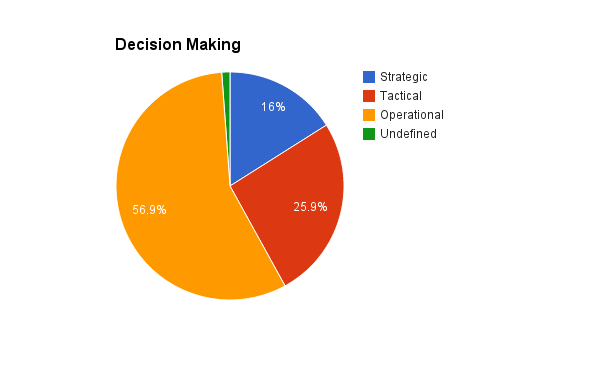
\includegraphics[width=\textwidth]{figures/decision-p.png}
	\caption{The distribution of different decision making decisions as they occurred over all the actions.}
	\label{figure:decision-p}
\end{figure}

\begin{figure}[!h]
	\centering
	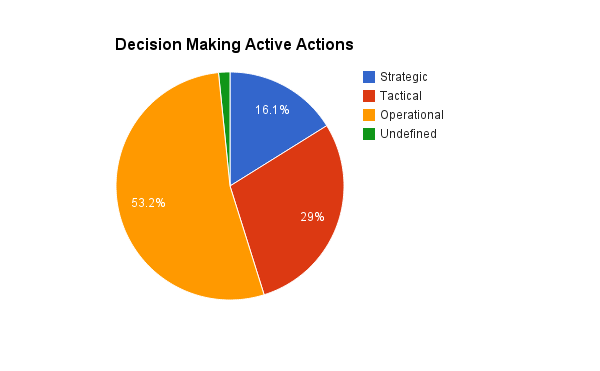
\includegraphics[width=\textwidth]{figures/decision-pa.png}
	\caption{The distribution of different decision making decisions as they occurred over the active actions.}
	\label{figure:decision-pa}
\end{figure}

\begin{sidewaysfigure}[!h]
	\centering
	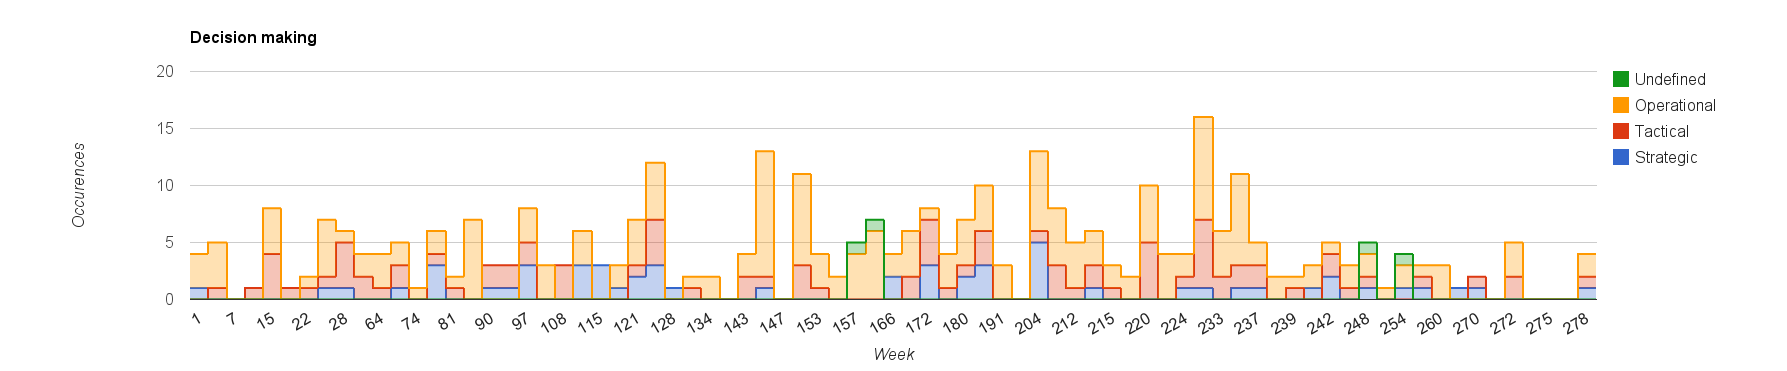
\includegraphics[width=\textwidth]{figures/decision-l.png}
	\caption{A timeline showing the distribution of the different decision making decisions for all the actions.}
	\label{figure:decision-l}
\end{sidewaysfigure}
\afterpage{\clearpage}

\subsubsection{Organizational Learning}
In terms of organizational learning each action could be defined as single-loop, double-loop or undefined. The results yielded from the content analysis showed that single-loop was the most occurring type of organizational learning with 66.4\% of the actions. Double-loop had 27.2\% of actions, and the rest was undefined at 6.4\%. The distribution over the timespan, \autoref{figure:learning-l} of the analysis showed that the three categories was evenly distributed. The active actions was very similar to the total amount of actions and only had some small negligible variances as can be seen in \autoref{figure:learning-p} and \autoref{figure:learning-pa}.

\begin{table}[!h]
	\begin{center}
	\caption{Results from the content analysis regarding the organizational learning nature of the action.}
	\label{table:organizational-learning-results}
	\makebox[\textwidth]{%
		\begin{tabular}{| l | l | l | l | l |}
		\hline
		Category & \multicolumn{2}{|c|}{All Actions} & \multicolumn{2}{|c|}{Active Actions}  \\
		\cline{2-5}
		& Number & Percentage & Number & Percentage \\	
		\hline
		Single-loop & 227 & 66.4\% & 41 & 66.1\% \\
		Double-loop & 93 & 27.2\% & 16 & 25.8\% \\
		Undefined & 22 & 6.4\% & 5 & 8.1\% \\
		\hline
		\end{tabular}
	}
	\end{center}
\end{table}

\begin{figure}[!h]
	\centering
	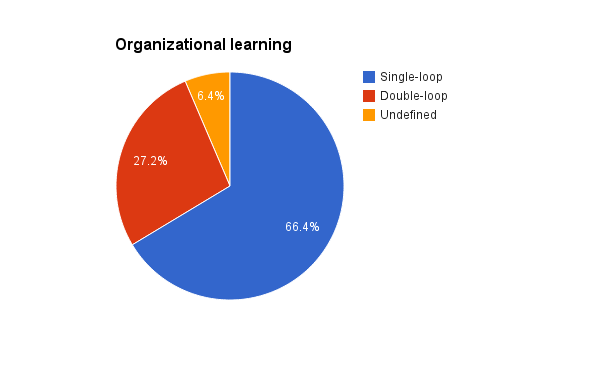
\includegraphics[width=\textwidth]{figures/learning-p.png}
	\caption{The distribution of single-loop, double-loop and undefined for all the actions.}
	\label{figure:learning-p}
\end{figure}

\begin{figure}[!h]
	\centering
	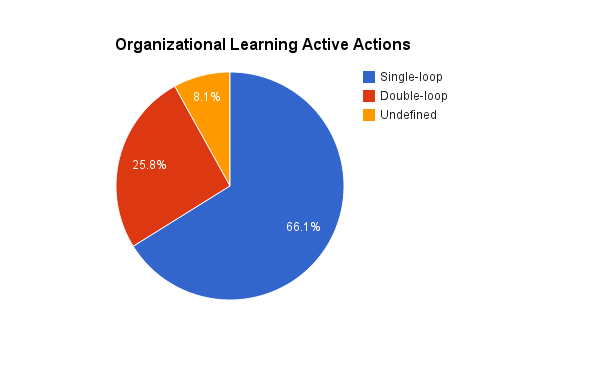
\includegraphics[width=\textwidth]{figures/learning-pa.png}
	\caption{The distribution of single-loop, double-loop and undefined for the active actions.}
	\label{figure:learning-pa}
\end{figure}

\begin{sidewaysfigure}[!h]
	\centering
	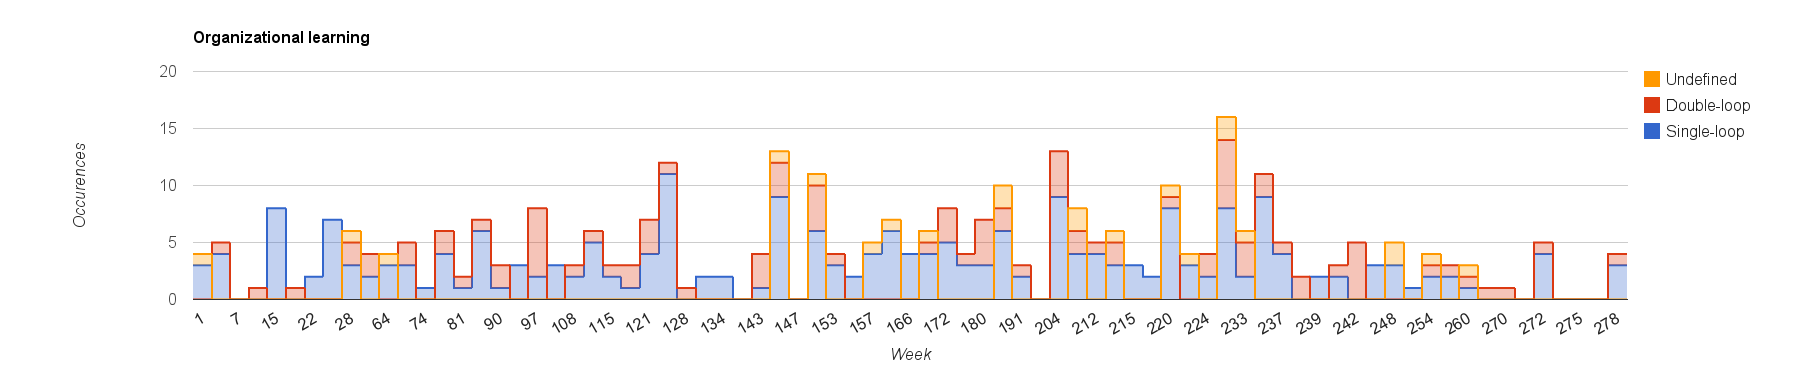
\includegraphics[width=\textwidth]{figures/learning-l.png}
	\caption{Timeline showing the distribution of learning loops for the total actions.}
	\label{figure:learning-l}
\end{sidewaysfigure}
\afterpage{\clearpage}

\subsubsection{Development Phase}

\begin{table}[!h]
	\begin{center}
	\caption{Results from the content analysis in which development phase the action regards.}
	\label{table:development-results}
	\makebox[\textwidth]{%
		\begin{tabular}{| l | l | l | l | l |}
		\hline
		Category & \multicolumn{2}{|c|}{All Actions} & \multicolumn{2}{|c|}{Active Actions}  \\
		\cline{2-5}
		& Number & Percentage & Number & Percentage \\	
		\hline
		Development & 89 & 18.4\% & 11 & 13.1\% \\
		Testing & 102 & 21.1\% & 18 & 21.4\% \\
		Documentation & 64 & 13.2\% & 16 & 19\% \\
		Release & 18 & 3.7\% & 4 & 4.8\% \\
		Build & 23 & 4.8\% & 6 & 7.1\% \\
		Business Development & 18 & 3.7\% & 5 & 6\% \\
		Planning & 119 & 24.6\% & 19 & 22.6\% \\
		Bugfix & 20 & 4.1\% & 2 & 2.4\% \\
		Undefined & 31 & 6.4\% & 3 & 3.6\% \\
		\hline
		\end{tabular}
	}
	\end{center}
\end{table}

\begin{figure}[!h]
	\centering
	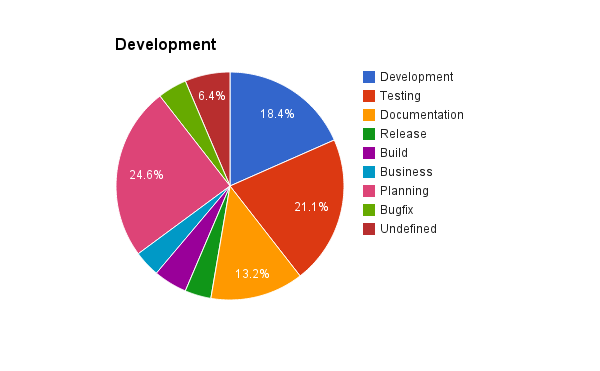
\includegraphics[width=\textwidth]{figures/development-p.png}
	\caption{The distribution of single-loop, double-loop and undefined for all the actions.}
	\label{figure:learning-p}
\end{figure}

\begin{figure}[!h]
	\centering
	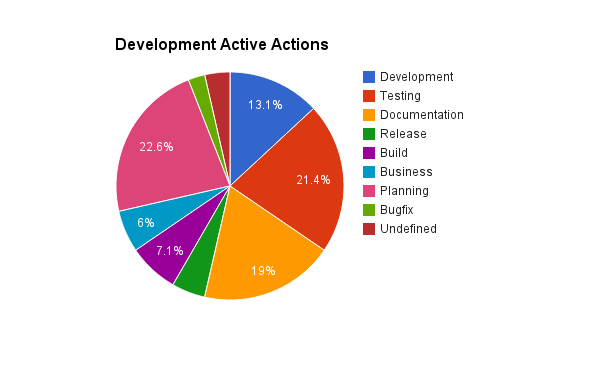
\includegraphics[width=\textwidth]{figures/development-pa.png}
	\caption{The distribution of single-loop, double-loop and undefined for the active actions.}
	\label{figure:learning-pa}
\end{figure}

\begin{sidewaysfigure}[!h]
	\centering
	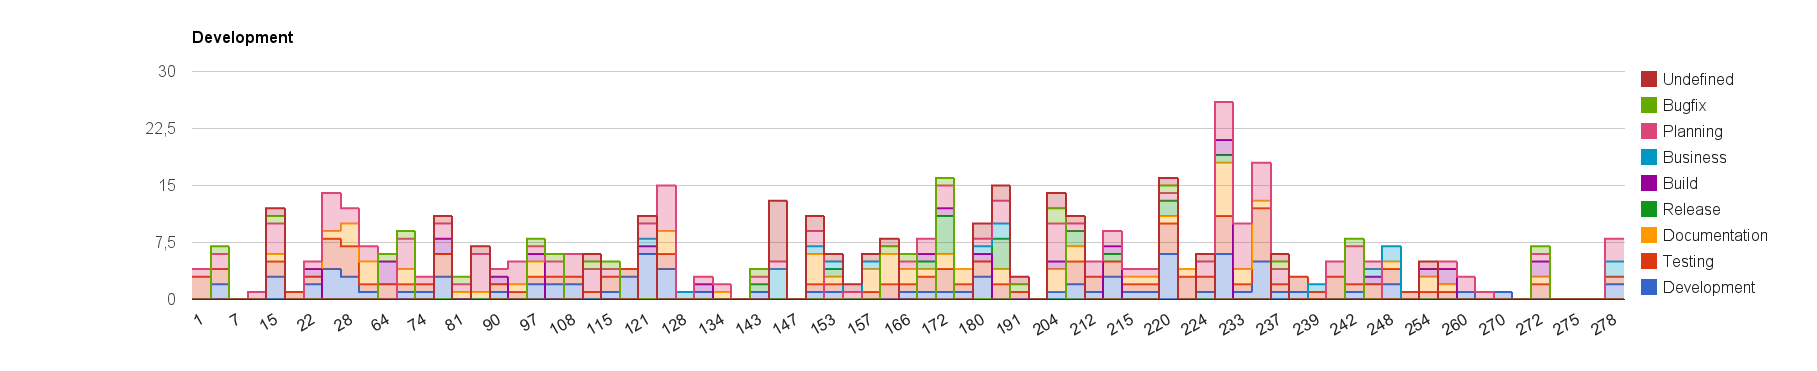
\includegraphics[width=\textwidth]{figures/development-l.png}
	\caption{Timeline showing the distribution of learning loops for the total actions.}
	\label{figure:learning-l}
\end{sidewaysfigure}
\afterpage{\clearpage}

\subsubsection{Collaboration}
\begin{table}[!h]
	\begin{center}
	\caption{Results from the content analysis regarding the collaboration influences of an action.}
	\label{table:collaboration-results}
	\makebox[\textwidth]{%
		\begin{tabular}{| l | l | l | l | l |}
		\hline
		Category & \multicolumn{2}{|c|}{All Actions} & \multicolumn{2}{|c|}{Active Actions}  \\
		\cline{2-5}
		& Number & Percentage & Number & Percentage \\	
		\hline
		Communication & 128 & 35.2\% & 14 & 20.9\% \\
		Leadership & 4 & 1.1\% & 1 & 1.5\% \\
		Competence & 25 & 6.9\% & 1 & 11.9\% \\
		External relations & 42 & 11.5\% & 11 & 16.4\% \\
		Undefined & 185 & 45.3\% & 33 & 48.3\% \\
		\hline
		\end{tabular}
	}
	\end{center}
\end{table}

\begin{figure}[!h]
	\centering
	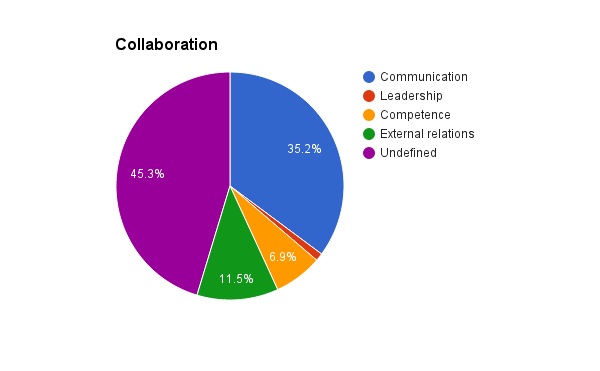
\includegraphics[width=\textwidth]{figures/management-p.png}
	\caption{The distribution of single-loop, double-loop and undefined for all the actions.}
	\label{figure:learning-p}
\end{figure}

\begin{figure}[!h]
	\centering
	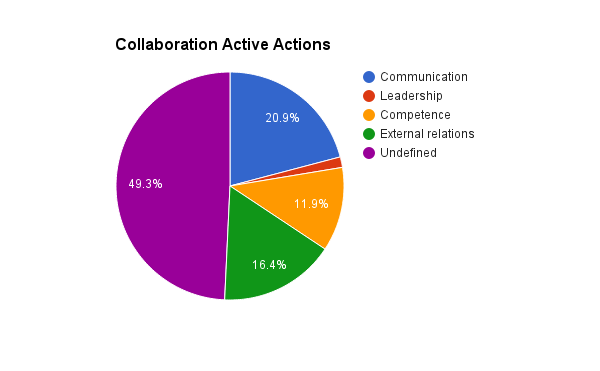
\includegraphics[width=\textwidth]{figures/management-pa.png}
	\caption{The distribution of single-loop, double-loop and undefined for the active actions.}
	\label{figure:learning-pa}
\end{figure}

\begin{sidewaysfigure}[!h]
	\centering
	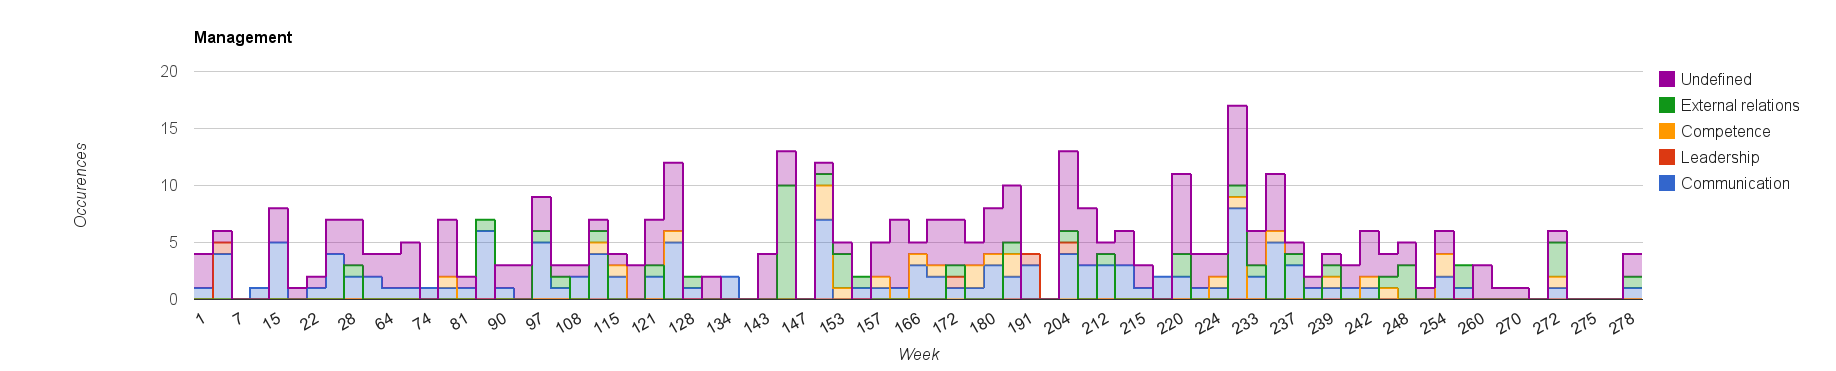
\includegraphics[width=\textwidth]{figures/management-l.png}
	\caption{Timeline showing the distribution of learning loops for the total actions.}
	\label{figure:learning-l}
\end{sidewaysfigure}
\afterpage{\clearpage}

\afterpage{\clearpage}